\documentclass[tikz,border=10pt]{standalone}
\usepackage{amsmath}
\usepackage{amssymb}
\usepackage{tikz}
\usetikzlibrary{arrows.meta,calc,decorations.pathreplacing,patterns,shapes.geometric,positioning,shadings}

\begin{document}
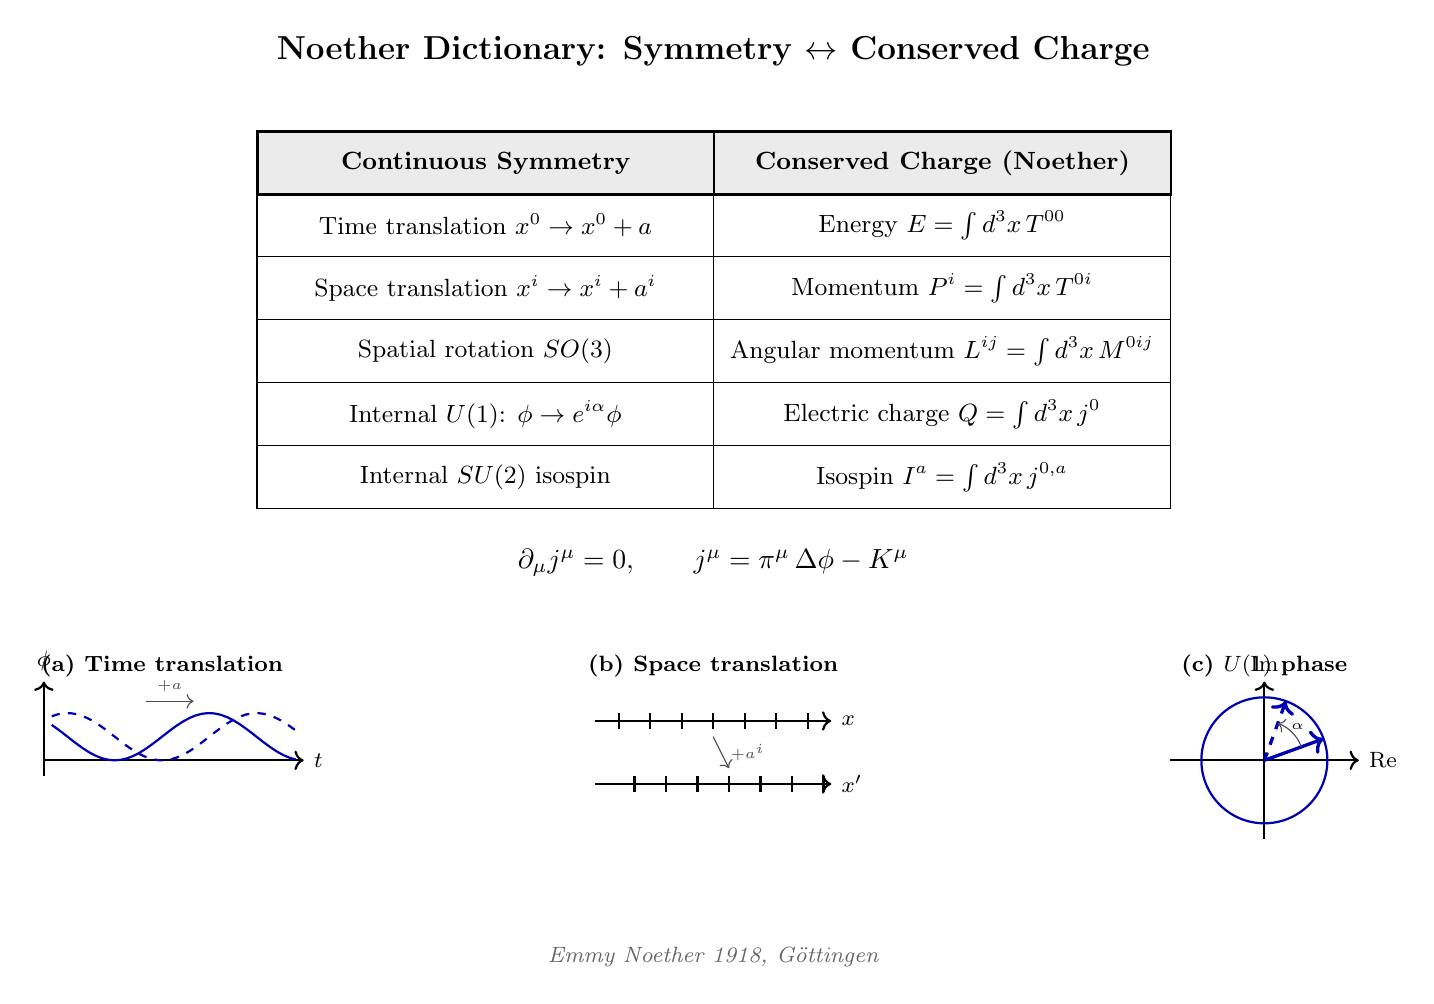
\begin{tikzpicture}[
    font=\small,
    headerstyle/.style={fill=black!8, draw=black, thick, minimum height=8mm, inner sep=3pt},
    cellL/.style={draw=black, thin, minimum height=8mm, minimum width=58mm, inner sep=3pt, anchor=west},
    cellR/.style={draw=black, thin, minimum height=8mm, minimum width=58mm, inner sep=3pt, anchor=west},
    smallnote/.style={font=\footnotesize, color=black!70}
]

% ============== Title ==============
\node[font=\bfseries\large] (title) at (0,0) {Noether Dictionary: Symmetry $\leftrightarrow$ Conserved Charge};

% ============== Table ==============
% Header row
\node[headerstyle, minimum width=58mm, anchor=north west] (hL) at (-58mm, -10mm) {\textbf{Continuous Symmetry}};
\node[headerstyle, minimum width=58mm, anchor=north west] (hR) at (0mm, -10mm) {\textbf{Conserved Charge (Noether)}};

% Row 1: Time translation -> Energy
\node[cellL, anchor=north west] (L1) at (-58mm, -18mm) {Time translation $x^0 \to x^0 + a$};
\node[cellR, anchor=north west] (R1) at (0mm, -18mm) {Energy $E = \int d^3x\, T^{00}$};

% Row 2: Space translation -> Momentum
\node[cellL, anchor=north west] (L2) at (-58mm, -26mm) {Space translation $x^i \to x^i + a^i$};
\node[cellR, anchor=north west] (R2) at (0mm, -26mm) {Momentum $P^i = \int d^3x\, T^{0i}$};

% Row 3: Rotation -> Angular momentum
\node[cellL, anchor=north west] (L3) at (-58mm, -34mm) {Spatial rotation $SO(3)$};
\node[cellR, anchor=north west] (R3) at (0mm, -34mm) {Angular momentum $L^{ij} = \int d^3x\, M^{0ij}$};

% Row 4: U(1) -> Charge
\node[cellL, anchor=north west] (L4) at (-58mm, -42mm) {Internal $U(1)$: $\phi \to e^{i\alpha}\phi$};
\node[cellR, anchor=north west] (R4) at (0mm, -42mm) {Electric charge $Q = \int d^3x\, j^0$};

% Row 5: SU(2) -> Isospin
\node[cellL, anchor=north west] (L5) at (-58mm, -50mm) {Internal $SU(2)$ isospin};
\node[cellR, anchor=north west] (R5) at (0mm, -50mm) {Isospin $I^a = \int d^3x\, j^{0,a}$};

% ============== Master formulas under table ==============
\node[anchor=north, font=\normalsize] (eq1) at (0mm, -62mm) {$\partial_\mu j^\mu = 0, \qquad j^\mu = \pi^\mu\, \Delta\phi - K^\mu$};

% ============== Three small diagrams below ==============
% (a) Time translation: two equivalent history curves
\begin{scope}[shift={(-70mm,-90mm)}, x=1mm, y=1mm]
  \node[font=\footnotesize\bfseries] at (0,12) {(a) Time translation};
  % axes
  \draw[->, thick] (-15,0) -- (18,0) node[right, font=\footnotesize] {$t$};
  \draw[->, thick] (-15,-2) -- (-15,10) node[above, font=\footnotesize] {$\phi$};
  % curve 1
  \draw[blue!70!black, thick] plot[domain=-14:17,samples=40] (\x, {3 + 3*sin(\x*15)});
  % curve 2 shifted
  \draw[blue!70!black, thick, dashed] plot[domain=-14:17,samples=40] (\x, {3 + 3*sin((\x-6)*15)});
  % shift arrow
  \draw[->, thin, black!70] (-2,7.5) -- (4,7.5) node[midway, above, font=\tiny] {$+a$};
\end{scope}

% (b) Space translation: coordinate ticks
\begin{scope}[shift={(0mm,-90mm)}, x=1mm, y=1mm]
  \node[font=\footnotesize\bfseries] at (0,12) {(b) Space translation};
  % top axis
  \draw[->, thick] (-15, 5) -- (15, 5) node[right, font=\footnotesize] {$x$};
  \foreach \x in {-12,-8,-4,0,4,8,12}
    \draw[thick] (\x, 4) -- (\x, 6);
  % bottom axis
  \draw[->, thick] (-15, -3) -- (15, -3) node[right, font=\footnotesize] {$x'$};
  \foreach \x in {-10,-6,-2,2,6,10,14}
    \draw[thick] (\x, -4) -- (\x, -2);
  % shift indicator
  \draw[->, thin, black!70] (0, 3) -- (2, -1) node[midway, right, font=\tiny] {$+a^i$};
\end{scope}

% (c) U(1) phase rotation in complex plane
\begin{scope}[shift={(70mm,-90mm)}, x=1mm, y=1mm]
  \node[font=\footnotesize\bfseries] at (0,12) {(c) $U(1)$ phase};
  % axes
  \draw[->, thick] (-12, 0) -- (12, 0) node[right, font=\footnotesize] {Re};
  \draw[->, thick] (0, -10) -- (0, 10) node[above, font=\footnotesize] {Im};
  % unit circle
  \draw[blue!70!black, thick] (0,0) circle [radius=8];
  % phase vector
  \draw[->, blue!70!black, very thick] (0,0) -- ({8*cos(20)}, {8*sin(20)});
  % rotated phase vector
  \draw[->, blue!70!black, very thick, dashed] (0,0) -- ({8*cos(70)}, {8*sin(70)});
  % rotation arc
  \draw[->, thin, black!70] ({5*cos(20)}, {5*sin(20)}) arc (20:70:5);
  \node[font=\tiny] at ({6*cos(45)}, {6*sin(45)}) {$\alpha$};
\end{scope}

% ============== Footnote ==============
\node[font=\footnotesize\itshape, color=black!60] at (0mm, -115mm) {Emmy Noether 1918, G\"ottingen};

\end{tikzpicture}
\end{document}
